\documentclass[11pt,compress,t,notes=noshow, aspectratio=169, xcolor=table]{beamer}
\newcommand{\btVFill}{\vskip0pt plus 1filll}
\newcommand\hmmax{0}
\newcommand\bmmax{0}
\usepackage{../../style/lmu-lecture}
\usepackage{siunitx}
% Defines macros and environments
% This file is included in slides and exercises

% Rarely used fontstyle for R packages, used only in 
% - forests/slides-forests-benchmark.tex
% - exercises/single-exercises/methods_l_1.Rnw
% - slides/cart/attic/slides_extra_trees.Rnw
\newcommand{\pkg}[1]{{\fontseries{b}\selectfont #1}}

% Spacing helpers, used often (mostly in exercises for \dlz)
\newcommand{\lz}{\vspace{0.5cm}} % vertical space (used often in slides)
\newcommand{\dlz}{\vspace{1cm}}  % double vertical space (used often in exercises, never in slides)
\newcommand{\oneliner}[1] % Oneliner for important statements, used e.g. in iml, algods
{\begin{block}{}\begin{center}\begin{Large}#1\end{Large}\end{center}\end{block}}

% Don't know if this is used or needed, remove?
% textcolor that works in mathmode
% https://tex.stackexchange.com/a/261480
% Used e.g. in forests/slides-forests-bagging.tex
% [...] \textcolor{blue}{\tfrac{1}{M}\sum^M_{m} [...]
% \makeatletter
% \renewcommand*{\@textcolor}[3]{%
%   \protect\leavevmode
%   \begingroup
%     \color#1{#2}#3%
%   \endgroup
% }
% \makeatother


\title{Interpretable Machine Learning}
% \author{LMU}
%\institute{\href{https://compstat-lmu.github.io/lecture_iml/}{compstat-lmu.github.io/lecture\_iml}}
\date{}

\begin{document}

% TODO
\newcommand{\titlefigure}{figure_man/exSHAP.png}
\newcommand{\learninggoals}{
  \item Recall order- and set-based definitions of Shapley values in ML
  \item Interpret predictions via additive Shapley decomposition
  \item Understand SHAP as surrogate-based model
  \item Understand SHAP properties
}

% \newcommand{\learninggoals}{
% \item Get an intuition of additive feature attributions
% \item Understand the concept of Kernel SHAP
% \item Ability to interpret SHAP plots
% \item Global SHAP methods
% }

\lecturechapter{SHAP (SHapley Additive exPlanation) Values}
\lecture{Interpretable Machine Learning}

% \begin{frame}{Shapley Values in ML - A short Recap}
  
%   \textbf{Question:} How much does a feat. $j$ contribute to the prediction of a single obs. \\
%   \textbf{Idea:} Use Shapley values from cooperative game theory \\
%   \pause
%   \textbf{Procedure:} 
%   \begin{itemize}
%     \item Compare ``reduced prediction function'' of feature coalition $S$ with $\Scupj$ 
%     \item Iterate over possible coalitions to calculate marginal contribution of feature $j$ to sample $\xv$
% \end{itemize}

% $$\phi_j 
% %= \frac{1}{|P|!} \sum_{\tau \in \Pi} (v(\Stauj) - v(\Stau)) 
% = \frac{1}{p!} \sum_{\tau \in \Pi}  \underbrace{\fh_{\Stauj}(\xv_{\Stauj}) - \fh_{\Stau}(\xv_{\Stau})}_{\text{marginal contribution of feature $j$}} $$

% \pause
% \textbf{Remember:}

% \begin{itemize}
%     \item $\fh$ is the prediction function, $p$ denotes the number of features
%     \item Non-existent feat. in a coalition are replaced by values of random feat. values 
%     \item Recall $\Stau$ defines the coalition as the set of players before player $j$ in order $\tau = (\tau^{(1)}, \dots, \tau^{(p)})$% states from the feature
    
%   \centerline{
%   \begin{tabular}{|c|c|c|c|c|c|c|}
%     %\multicolumn{3}{c}{\enspace\raisebox{-3.3ex}[0pt][2.6ex]{$ \overbrace{\vphantom{-}\hspace{9em}}^{|S|! \text{ permutations}}$}} &
%     %\multicolumn{1}{c}{} &
%     %\multicolumn{3}{c}{\enspace\raisebox{-3.3ex}[0pt][2.6ex]{$ \overbrace{\vphantom{-}\hspace{9em}}^{(|P| - |S| - 1)! \text{ permutations}}$}}\\
%     \hline
%     $\tau^{(1)}$ & \ldots & $\tau^{(|S|)}$ & $\tau^{(|S| + 1)}$ & $\tau^{(|S| + 2)}$ & \ldots & $\tau^{(p)}$ \\
%     \hline
%     \multicolumn{3}{c}{\enspace\raisebox{1.3ex}[0pt][2.6ex]{$ \underbrace{\vphantom{-}\hspace{9em}}^{}$}} &
%     \multicolumn{1}{c}{\enspace\raisebox{1.3ex}[0pt][2.6ex]{$ \underbrace{\vphantom{-}\hspace{4em}}^{}$}} &
%     \multicolumn{3}{c}{\enspace\raisebox{1.3ex}[0pt][2.6ex]{$ \underbrace{\vphantom{-}\hspace{9em}}^{}$}}\\
%     \multicolumn{3}{c}{$S_j^\tau:$ Players before player $j$} & \multicolumn{1}{c}{player $j$} & \multicolumn{3}{c}{Players after player $j$} \\
%   \end{tabular}}
% \end{itemize}

% \end{frame}


\begin{frame}{Shapley Values in ML - A Short Recap}

% \textbf{Question:} How much does $x_j$ contribute to prediction of a specific obs. $\xv$?
% 
% \textbf{Idea:} Use Shapley values to compute fair attributions.
% 
% \pause
\textbf{Shapley values (order definition):} Average over marginal contributions across all permutations of feature indices $\tau \in \Pi$:

\[
\phi_j(\xv) = \frac{1}{p!} \sum_{\tau \in \Pi} 
\underbrace{\fh_{\Stauj}(\xv_{\Stauj}) - \fh_{\Stau}(\xv_{\Stau})}_{\text{marginal contribution of feature $j$}}
\]

%\pause
%\textbf{Procedure:}
\begin{itemize}
  \item For each permutation $\tau$, determine coalition $\Stau$: features before $j$ in $\tau$
  \item In \(\fh_S\), features not in \(S\) are marginalized (e.g., replaced by random imputations)
  %$\leadsto$ In practice, features not in \(S\) are 
  \item Compute marginal contribution of adding $j$ to $\Stau$ via the difference above
  \item Average over all $p!$ permutations (in practice, over $M << p!$)
\end{itemize}

\pause\medskip

\textbf{Alternative (set definition):} Average marginal contribution over all subsets, weighted by their relative number of appearances in permutations:

\[
\phi_j(\xv) = 
\sum_{S \subseteq \{1,\dots,p\} \setminus \{j\}} \frac{|S|!(p - |S| - 1)!}{p!} \left[\fh_{S \cup \{j\}}(\xv_{S \cup \{j\}}) - \fh_S(\xv_S)\right].
\]
% 
% \pause
% \textbf{Notes:}
% \begin{itemize}
%   \item $\fh$: prediction function; $p$: number of features
%   \item Features not in the coalition are replaced via marginalization (e.g., random imputations of feature values)
% \end{itemize}
% 
% \vspace{0.4em}
% \centerline{
% \begin{tabular}{|c|c|c|c|c|c|c|}
%   \hline
%   $\tau^{(1)}$ & $\cdots$ & $\tau^{(|S|)}$ & $\tau^{(|S|+1)}$ & $\tau^{(|S|+2)}$ & $\cdots$ & $\tau^{(p)}$ \\
%   \hline
%   \multicolumn{3}{c}{$\underbrace{\hspace{9em}}_{\Stau}$} & 
%   \multicolumn{1}{c}{$\underbrace{\hspace{4em}}_{j}$} & 
%   \multicolumn{3}{c}{$\underbrace{\hspace{9em}}_{\text{Remaining features}}$}
% \end{tabular}
% }

\end{frame}

% 
% \begin{frame}{Shapley Values in ML - A short Recap}
%   
%   \textbf{Example:} Random forest trained on bike share data using only humidity (hum), temperature (temp), windspeed (ws)
% \begin{columns}[T, onlytextwidth]
% \begin{column}{0.58\textwidth}
% 
%   \begin{itemize}
%       \item Observation $\xv$ with prediction $\fh(\xv) = \color{orange}{2573}$
%       \item Mean prediction $\E(\fh) = \color{blue}{4515}$
%   \end{itemize}
%   
%   \medskip
%   
%   
%   \textbf{Exact Shapley value for hum:} 
%       {\centering
%       \scriptsize
%       \begin{tabular}{c|c|c|c|c}
%    $S$    &  $\Scupj$  & $\fh_S$ &  $\fh_{\Scupj}$  & weight\\\hline
%      $\varnothing$&    hum  & \color{blue}{4515} & 4635 & $2/6$\\
%        temp &  temp, hum & 3087 & 3060& $1/6$\\
%        ws &  ws, hum & 4359  & 4450 & $1/6$\\
%        temp, ws & temp, ws, hum & 2623 & \color{orange}{2573} & $2/6$
%       \end{tabular}
%       }
% \end{column}
% \begin{column}{0.42\textwidth}
% %\vspace{-1cm}
% 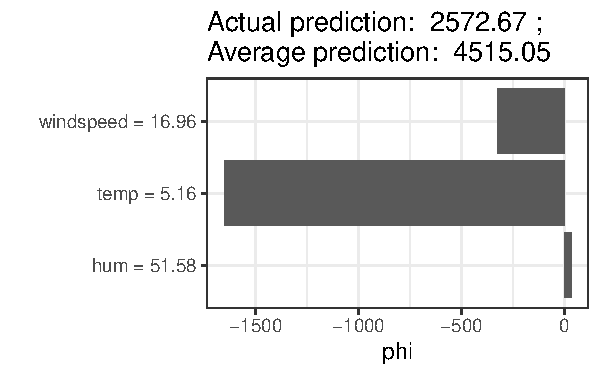
\includegraphics[width=\linewidth]{figure/shapley2shap.pdf}
% \end{column}
% \end{columns}
% 
% $$\Rightarrow
% \phi_{hum} = \tfrac{2}{6} (4635-4515) + \tfrac{1}{6} (3060-3087) + \tfrac{1}{6} (4450-4359) + \tfrac{2}{6} (2573-2623) = 34
% $$
% $\Rightarrow$ Analogously $\phi_{\text{temp}} = -1654$, $\phi_{\text{ws}} = -322$
% % \begin{align*}
% %  v(P) &= \fh(\xv) - \E(\fh) = \phi_{\text{hum}} + \phi_{\text{temp}} + \phi_{\text{ws}} \\
% %  &= {\color{orange} 2573} - {\color{blue} 4515} = 34 - 1654 - 322 = -1942
% %  \end{align*}
% 
% \medskip
% 
% \textbf{Interpretation:} \texttt{hum} raises prediction by 34, \texttt{temp} and \texttt{ws} lower it by 1654 and 322, explaining the deviation from the mean
% 
% %\textbf{Recall:} Shapley values explain how features shift prediction from baseline $\E(\fh)$:
% % \begin{align*}
% % v(P) &= \fh(\xv) - \E(\fh) = \phi_{\text{hum}} + \phi_{\text{temp}} + \phi_{\text{ws}} \\
% % &= {\color{orange} 2573} - {\color{blue} 4515} = 34 - 1654 - 322 = -1942
% % \end{align*}
% 
% \end{frame}



\begin{frame}{Shapley Values in ML - Example}
  
  \textbf{Example (Bike sharing data):}

  \begin{itemize}
  \item Train random forest using humidity (hum), temperature (temp), windspeed (ws)
      \item Consider observation of interest $\xv$ with prediction $\fh(\xv) = \color{orange}{2573}$
      \item Mean prediction $\E_{\xv}[\fh(\xv)] = \color{blue}{4515}$
      \item Compute exact Shapley value for $\xv$ for feature hum:
  \end{itemize}
  
      \begin{center}
      \begin{tabular}{c|c|c|c|c}
   $S$    &  $\Scupj$  & $\fh_S$ &  $\fh_{\Scupj}$  & weight\\\hline
     $\varnothing$&    hum  & \color{blue}{4515} & 4635 & $2/6$\\
       temp &  temp, hum & 3087 & 3060& $1/6$\\
       ws &  ws, hum & 4359  & 4450 & $1/6$\\
       temp, ws & temp, ws, hum & 2623 & \color{orange}{2573} & $2/6$
      \end{tabular}
      \end{center}
$$\Rightarrow
\phi_{\text{hum}}(\xv) = \tfrac{2}{6} (4635-4515) + \tfrac{1}{6} (3060-3087) + \tfrac{1}{6} (4450-4359) + \tfrac{2}{6} (2573-2623) = 34
$$
$\Rightarrow$ Analogously $\phi_{\text{temp}}(\xv) = -1654$, $\phi_{\text{ws}}(\xv) = -322$
% \begin{align*}
%  v(P) &= \fh(\xv) - \E(\fh) = \phi_{\text{hum}} + \phi_{\text{temp}} + \phi_{\text{ws}} \\
%  &= {\color{orange} 2573} - {\color{blue} 4515} = 34 - 1654 - 322 = -1942
%  \end{align*}

\end{frame}

% 
% \begin{frame}{From Shapley to SHAP}
% \textbf{Example continued}: Same calculation can be done for temperature and windspeed:
% \begin{itemize}
%     \item $\phi_{temp} = \ldots = -1654$
%     \item $\phi_{ws} = \ldots = -322$
% \end{itemize}
% 
% \textbf{Remember}: Shapley values explain difference between actual and average pred.:
% \begin{eqnarray*}
% \color{orange}{2573} \color{black}- \color{blue}{4515} \color{black} &= 34 - 1654 - 322 &= - 1942\\
% \fh(\xv) - \E(\fh) &= \phi_{hum} + \phi_{temp} + \phi_{ws}&\\
% \end{eqnarray*}
% \begin{columns}[T]
% \begin{column}{0.5\textwidth}
% $\leadsto$ can be rewritten as
% $$
% \fh(\xv) = \underbrace{\E(\fh)}_{\phi_0} + \phi_{hum} + \phi_{temp} + \phi_{ws}
% $$
% $\leadsto$ Additive decomposition: baseline $\phi_0$ + per-feature contributions $\phi_j$
% %N.B.: This reminds us of a LM with weights $\phi_j$ multiplied by a binary feature value indicating weather a feature is included in a considered coalition.
% \end{column}
% \begin{column}{0.5\textwidth}
% \vspace{-1cm}
% \begin{figure}
%     \centering
%     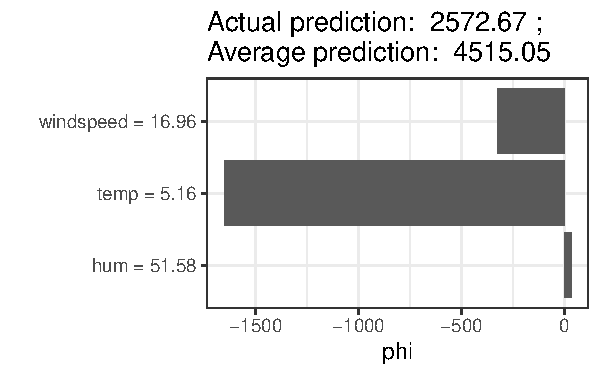
\includegraphics[width=0.9\columnwidth]{figure/shapley2shap.pdf}
% \end{figure}
% \end{column}
% \end{columns}
% \end{frame}

\begin{frame}{From Shapley Values to SHAP}


\begin{columns}[T, onlytextwidth]
\begin{column}{0.51\textwidth}

%\textbf{Example (cont.):} Shapley values for other features $\phi_{\text{temp}} = -1654$, $\phi_{\text{ws}} = -322$

%\medskip

% \textbf{Interpretation:} \texttt{hum} raises prediction by 34, \texttt{temp} and \texttt{ws} lower it by 1654 and 322, explaining the deviation from the mean

% \medskip
\textbf{Shapley value interpretation (for $\xv$):}
\begin{itemize}
  \item \texttt{hum} \(\;(+34)\) pushes prediction \emph{above} baseline (= average prediction).  
  \item \texttt{temp} \(\;(-1654)\) and \texttt{ws} \(\;(-322)\) pull prediction \emph{below} baseline.
  \item Together, they explain full deviation from average prediction.
\end{itemize}

%\medskip


% \textbf{Recall:} Shapley values explain how features shift prediction from baseline $\E(\fh)$:
% \footnotesize
% \begin{align*}
%  \fh(\xv) - \E_{\xv}[\fh(\xv)] &= \phi_{\text{hum}}(\xv) + \phi_{\text{temp}}(\xv)  + \phi_{\text{ws}}(\xv) \\
%  {\color{orange} 2573} - {\color{blue} 4515} &= 34 - 1654 - 322 = -1942
% \end{align*}

\end{column}
\begin{column}{0.49\textwidth}
%\vspace{-1cm}
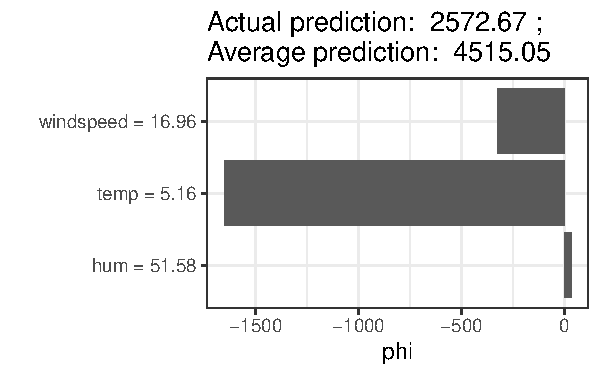
\includegraphics[trim={10 17 5 5},clip, width=\linewidth]{figure/shapley2shap.pdf}
\end{column}
\end{columns}
\pause
\textbf{Shapley-based additive decomposition} of prediction for $\xv$ gives insights on how features shift prediction from baseline $\E(\fh)$:

\medskip

\centerline{$
\underbrace{{\color{orange} \fh(\xv)}}_{\text{actual prediction}}
={\color{blue} \underbrace{\phi_0}_{\E_{\mathbf X}[\fh(\mathbf X)]}}
+\sum_{j\in\{\text{hum},\text{temp},\text{ws}\}}\phi_j(\xv)
$}
%\footnotesize
\medskip
\centerline{$
\phantom{=} \; {\color{orange} 2573}
= {\color{blue} 4515}
\;+\;
\bigl(34 -1654 - 322\bigr)
\;=\;4515-1942
$}
\medskip

\(\leadsto\) Like a LM evaluated at \(\xv\): global intercept \(\phi_0\) plus per-feature contributions \(\phi_j(\xv)\).

\medskip
%\vspace{0.4em}
% \textbf{SHAP:} Express prediction of $\xv$ as additive decomposition of Shapley values
% \[
% \fh(\xv) = \underbrace{\E(\fh)}_{\phi_0} + \sum_j \phi_j
% \]
% $\leadsto$ Analogous to linear models: intercept $\phi_0$ + per-feature contributions $\phi_j$

% \textbf{SHAP takeaway:}  
% \[
% \fh(\xv)=\underbrace{\E_{\xv}[\fh(\xv)]}_{\phi_0}
%       +\sum_{j=1}^{p}\phi_j(\xv)
%       \quad\text{with each }\phi_j(\xv)\text{ the \emph{Shapley value} of feature }j.
% \]

%\(\leadsto\) Like a linear model evaluated at \(\xv\): global intercept \(\phi_0\) plus instance-specific feature contributions \(\phi_j(\xv)\).

\textbf{SHAP Motivation:}
Can we efficiently estimate this Shapley-based additive decomposition of $\fh(\xv)$ using a surrogate model (while preserving Shapley axioms)?

%Additive explanation model: intercept $\phi_0$ plus per-feature effects $\phi_j$ (analogous to a linear model)
%Reminds of linear models: $\phi_j$ as effect of feature $j$ and intercept $\phi_0$ 
\end{frame}



% 
% \begin{frame}{From Shapley Values to the SHAP}
% 
% SHAP defines an \textbf{additive local surrogate model} \(g(\mathbf{z}^{\prime})\) based on a binary \textbf{simplified input} \(\mathbf{z}^{\prime} = (z^{\prime}_1, \dots, z^{\prime}_p)^\top \in \{0,1\}^p\), where:
% \[
% g(\mathbf{z}^{\prime}) = \phi_0 + \sum_{j=1}^p \phi_j z^{\prime}_j
% \]
% \begin{itemize}
%   \item \(z^{\prime}_j = 1\): feature \(j\) is "observed" (i.e., present in coalition)
%   \item \(z^{\prime}_j = 0\): feature \(j\) is "absent" and replaced via (conditional) imputation
%   \item SHAP seeks \(\phi_j\) values such that Shapley axioms hold %$\Rightarrow$ guarantees fairness, consistency, and efficiency.
% \end{itemize}
% \end{frame}
% % 
% % \begin{frame}{From Shapley to SHAP Model}
% % 
% % SHAP defines an additive feature attribution model (local surrogate model) \(g(\mathbf{z}^{\prime})\) based on a simplified feature vector \(\mathbf{z}^{\prime}\in\{0,1\}^p\) indicating whether a feature value was replaced by random imputation:
% % \[
% %  g(\mathbf{z}^{\prime})=\phi_0+\sum_{j=1}^p\phi_j z^{\prime}_j
% % \]
% % \begin{itemize}
% %   \item $z^{\prime}_j=1$ feature present; $z^{\prime}_j = 0$ replaced by random imputation.
% %   \item Find coefficients \(\phi_j\) such that Shapley axioms hold \(\Rightarrow\) SHAP.
% % \end{itemize}
% % \end{frame}
% 
% 
% \begin{frame}{SHAP Definition \citebutton{Lundberg et al. 2017}{https://doi.org/10.48550/arXiv.1705.07874}}
% \textbf{Aim}: 
% %Find an additive combination that explains the prediction of an observation $\xv$ by computing the contribution of each feature to the prediction using a (more efficient) estimation procedure. \\\medskip
% Explain a prediction $\fh(\xv)$ by decomposing it into additive contributions from individual features using a surrogate model and efficient Shapley estimation.
% 
% \medskip
% 
% \only<1-5>{\textbf{SHAP Setup}
% \begin{itemize}
%     % \item Simplified (binary) coalition feat. space $\mathbf{Z}^\prime \in \{0,1\}^{K \times p}$ with $K$ rows and $p$ cols.
%     % \item Rows are referred to as $\mathbf{z}^{\prime (k)} = \{z^{\prime (k)}_1, \ldots, z^{\prime (k)}_p\}$ with $k \in \{1,\ldots, K\}$ (indexes $k$-th coalition)
%     % \item Cols are referred to as $\mathbf{z}_j$ with $j \in \{1, \ldots, p\}$ being the index of the original feat.
%      \item Simplified (binary) coalition feat. space $\mathbf{Z}^\prime \in \{0,1\}^{K \times p}$ with $K$ rows and $p$ cols.
%     \item Each row $\mathbf{z}^{\prime (k)} = (z_1^{\prime(k)}, \ldots, z_p^{\prime(k)})$ represents a coalition (subset of features).
%     \item Each column $\mathbf{z}_j$ indicates if feature $j$ is part of a coalition.
% \end{itemize}
% }
% 
% \medskip
% 
% \only<1>{
% \textbf{Example -- Coalition Space for 3 Features}: 
% \vspace{-0.2cm}
% \begin{table}[]
%     \centering
%     \footnotesize
%      \begin{tabular}{l |c|ccc}
%   Coalition  & $\mathbf{z}^{\prime (k)}$ &  hum & temp & ws \\
%   \hline 
%   $\varnothing$ & $\mathbf{z}^{\prime (1)}$ & 0 & 0 & 0  \\
%   hum & $\mathbf{z}^{\prime (2)}$ & 1 & 0 & 0  \\
%   temp &  $\mathbf{z}^{\prime (3)}$ & 0 & 1 & 0  \\
%   ws &   $\mathbf{z}^{\prime (4)}$ & 0 & 0 & 1  \\
%   hum, temp & $\mathbf{z}^{\prime (5)}$ & 1 & 1 & 0  \\
%   temp, ws & $\mathbf{z}^{\prime (6)}$ & 0 & 1 & 1  \\
%   hum, ws &   $\mathbf{z}^{\prime (7)}$ & 1 & 0 & 1  \\
%   hum, temp, ws & $\mathbf{z}^{\prime (8)}$ & 1 & 1 & 1  \\
%   \end{tabular}
% \end{table}
% }
% \only<2->{
% %\vspace{0.5cm}
% \begin{exampleblock}{}
% \[
% g\left(\tikzmark{zp} \mathbf{z}^{\prime (k)}\right)=
% \tikzmark{ph0}\phi_{0}+\sum_{j=1}^{p}
% \tikzmark{phj} \phi_{j} z_{j}^{\prime (k)}
% \]
% \begin{tikzpicture}[
%   remember picture,
%   overlay,
%   expl/.style={draw=blue,fill=white,rounded corners,text width=3cm},
%   arrow/.style={blue,ultra thick,->,>=latex}
% ]
% \node<2-4>[expl] 
%   (zex) 
%   at (2,1.5cm)
%   {$\mathbf{z}^{\prime (k)}$: \textbf{Coalition} \\ simplified features};
% \node<3-4>[expl] 
%   (ph0ex) 
%   at (4,-.5cm)
%   {$\phi_0$: \textbf{Null Output} \\ Average Model Baseline ($\E(\fh))$};
% \node<4>[expl] 
%   (phjex) 
%   at (10,0cm)
%   {$\phi_j$: \textbf{Attribution} \\ How much does feature $j$ change the output for coalition $k$};
% 
% \draw<2-4>[arrow]
%   (zex.east) to[out=0,in=120] ([xshift= 1ex, yshift=2.3ex]{pic cs:zp});  
% \draw<3-4>[arrow]
%   (ph0ex.east) to[out=0,in=270] ([xshift= 1ex, yshift=-0.8ex]{pic cs:ph0});  
% \draw<4>[arrow]
%   (phjex.west) to[out=180,in=270] ([xshift= 1ex, yshift=-1ex]{pic cs:phj});
%  \node<5>[expl] 
%   (zex)  
%   at (2,1cm)
%   {$g(\mathbf{z}^{\prime (k)})$: \textbf{Marginal Contribution} \\ Contribution of coalition $\mathbf{z}^{\prime (k)}$ to the prediction};
%   \draw<5>[arrow]
%   (zex.east) to[out=0,in=140] ([xshift= 1ex, yshift=2.3ex]{pic cs:zp});  
% \node<5>[expl] 
%   (phjsh) 
%   at (10,1.5cm)
%   {$\phi_j$: \textbf{Shapley Values}};
% \draw<5>[arrow]
%   (phjsh.west) to[out=180,in=50] ([xshift= 1ex, yshift=2ex]{pic cs:phj}); 
% \draw<5> [
%     thick,
%     decoration={
%         brace,
%         mirror,
%         raise=0.5cm
%     },
%     decorate
% ] (5.7,0.7) -- (8.2,0.7)
% node[pos=0.5,below=15pt,black]{\textbf{Additive Feature Attribution}};
% \end{tikzpicture}
% \end{exampleblock}
% \begin{onlyenv}<5>
% \vspace{1cm}
% \textbf{Next:} How do we estimate the Shapley values $\phi_j$ efficiently?
% \end{onlyenv}}
% 
% \end{frame}

\begin{frame}{SHAP Framework \citebutton{Lundberg et al. 2017}{https://doi.org/10.48550/arXiv.1705.07874}}

\textbf{SHAP} expresses the prediction of $\xv$ as a sum of contributions from each feature:

\[
g(\zv') = \phi_0 + \textstyle\sum_{j=1}^p \phi_j z'_j
\]

\begin{itemize}
  \item $\zv' \in \{0,1\}^p$: simplified binary input referring to a coalition (coalition vector)
  \item \(z'_j = 1\): feature $j$ is "present" $\Rightarrow$ use $x_j$ in model evaluation
  \item \(z'_j = 0\): feature $j$ is "absent"\\$\Rightarrow$ influence of $x_j$ is removed via marginalization over a reference distribution% (averaging predictions over its possible values, given the present features)%\\
  %$\leadsto$ \textit{Note: In practice (e.g., KernelSHAP), marginalization is approximated via random imputations from background data.}
\end{itemize}

\pause\medskip

\textbf{SHAP as a theoretical framework:} Fit a surrogate model \( g(\zv') \) satisfying Shapley axioms and recovering $\fh(\xv)$ when all features are "present":
%Construct a surrogate model $g(\zv')$ such that it satisfies the Shapley value axioms and recovers $\fh(\xv)$ when all features are "present":
\[
\fh(\xv) = g(\mathbf{1}) = \phi_0 + \textstyle\sum_{j=1}^p \phi_j
\]
\textbf{Evaluation of $g(\zv')$:} Let \( S = \{ j : z'_j = 1 \} \) be the active coalition. Then:
\begin{itemize}
    \item $g(\zv') \approx \mathbb{E}[ \fh(\mathbf{X}) \mid \mathbf{X}_S = \mathbf{x}_S]\;\text{(conditional expectation)}$
    \item $g(\zv') \approx \mathbb{E}_{\mathbf{X}_{-S}} [ \fh(\mathbf{x}_S, \mathbf{X}_{-S}) ] \;\;\text{(marginal expectation, i.e., PD function)}$
    \item\textit{Note: Practical implementations (e.g., KernelSHAP) use the marginal expectation, approximated via random imputations from background data.}
\end{itemize}

\end{frame}


% \begin{frame}{SHAP Framework \citebutton{Lundberg et al. 2017}{https://doi.org/10.48550/arXiv.1705.07874}}

% \textbf{SHAP} expresses the prediction of $\xv$ as a sum of contributions from each feature:

% \[
% g(\zv') = \phi_0 + \sum_{j=1}^p \phi_j z'_j
% \]

% \begin{itemize}
%   \item $\zv' \in \{0,1\}^p$: simplified binary input referring to a coalition (coalition vector)
%   \item \(z'_j = 1\): feature $j$ is "present" $\Rightarrow$ use $x_j$ in the model evaluation
%   \item \(z'_j = 0\): feature $j$ is "absent" $\Rightarrow$ marginalize $x_j$ (average over its possible values)\\
%   $\leadsto$ \textit{Note: In practice (e.g., KernelSHAP), marginalization is approximated via random imputations from background data.}
% \end{itemize}

% \vspace{0.5em}
% \textbf{Key idea:} Construct a surrogate model $g(\zv')$ such that it satisfies the Shapley value axioms and recovers $\fh(\xv)$:
% \[
% \fh(\xv) = g(\mathbf{1}) = \phi_0 + \sum_{j=1}^p \phi_j
% \]


% \end{frame}


% \begin{frame}{SHAP Framework \citebutton{Lundberg et al. 2017}{https://doi.org/10.48550/arXiv.1705.07874}}

% \textbf{SHAP} defines a surrogate \(g(\zv')\) over binary vectors \(\zv' \in \{0,1\}^p\) (simplified features):

% \[
% g(\zv') = \phi_0 + \sum_{j=1}^p \phi_j z'_j
% \]

% \begin{itemize}

%   \item \textbf{Fixed:} \(\xv\) is the instance being explained (i.e., SHAP explains \(\fh(\xv)\))
%   \item \textbf{Coalitions:} \(\zv'\) encodes which features of \(\xv\) are "observed" in coalition:
%     \begin{itemize}
%       \item \(z'_j = 1\): feature \(j\) is included $\Rightarrow$ use \(x_j\)
%       \item \(z'_j = 0\): feature \(j\) is excluded $\Rightarrow$ \(x_j\) is marginalized out
%       %random imputation when evaluating \(\fh\)
%     \end{itemize}
% \item Each $\zv'$ represents a \textbf{feature coalition} used to approximate $\fh(\xv)$\\
% %Each \(\zv'\) represents a \textbf{coalition}, i.e., a subset of features considered "known" for the prediction at \(\xv\)
%   %\item Many different \(\zv'\) are used for the same \(\xv\), to simulate all possible feature subsets and compute marginal contributions.
%   $\leadsto$ Many \(\zv'\) are constructed from \(\xv\), defining a subset of "observed" features\\
%   $\leadsto$ Used to estimate marginal contributions and compute Shapley values
%   \item SHAP computes \(\phi_j\) such that \(g(\zv')\) satisfies Shapley axioms and recovers \(\fh(\xv)\)
%   %SHAP chooses the \(\phi_j\) such that \(g(\zv')\) approximates \(\fh(\xv)\) in a way that satisfies the Shapley axioms.
% \end{itemize}


%  \end{frame}

\begin{frame}{SHAP Framework \citebutton{Lundberg et al. 2017}{https://doi.org/10.48550/arXiv.1705.07874}}

%\textbf{Goal:} Explain a prediction \(\fh(\xv)\) by decomposing it into additive feature contributions using a local surrogate model derived from Shapley values.

\medskip

\textbf{SHAP}  
defines an additive surrogate \(g(\zv')\) over a binary simplified input \(\zv' \in \{0,1\}^p\):
% \only<1>{
% \[
% g(\zv') = \phi_0 + \sum_{j=1}^p \phi_j z'_j
% \]
% \begin{itemize}
%   \item \(z'_j = 1\): feature \(j\) is "observed" (included in coalition)
%   \item \(z'_j = 0\): feature \(j\) is "absent" and replaced via (conditional) imputation
%   \item \(\phi_j\): contribution of feature \(j\) to \(\fh(\xv)\), satisfying Shapley axioms
% \end{itemize}

% \medskip

% \textbf{Coalition space:} each row \(\zv'^{(k)} \in \{0,1\}^p\) refers to a coalition

% \begin{table}[]
%     \centering
%     \footnotesize
%      \begin{tabular}{l |c|ccc}
%   Coalition  & $\zv'^{(k)}$ &  hum & temp & ws \\
%   \hline 
%   $\varnothing$ & $\zv'^{(1)}$ & 0 & 0 & 0  \\
%   hum & $\zv'^{(2)}$ & 1 & 0 & 0  \\
%   temp &  $\zv'^{(3)}$ & 0 & 1 & 0  \\
%   ws &   $\zv'^{(4)}$ & 0 & 0 & 1  \\
%   hum, temp & $\zv'^{(5)}$ & 1 & 1 & 0  \\
%   temp, ws & $\zv'^{(6)}$ & 0 & 1 & 1  \\
%   hum, ws &   $\zv'^{(7)}$ & 1 & 0 & 1  \\
%   hum, temp, ws & $\zv'^{(8)}$ & 1 & 1 & 1  \\
%   \end{tabular}
% \end{table}
% }

\only<1->{
\begin{exampleblock}{}
\[
g\left(\tikzmark{zp} \zv'^{(k)}\right) =
\tikzmark{ph0} \phi_0 + \sum_{j=1}^p \tikzmark{phj} \phi_j z_j'^{(k)}
\]
\begin{tikzpicture}[
  remember picture,
  overlay,
  expl/.style={draw=blue,fill=white,rounded corners,text width=3.5cm},
  arrow/.style={blue,ultra thick,->,>=latex}
]
\node<1>[expl] (zex) at (2,1.5cm)
  {\(\zv'^{(k)}\): \textbf{coalition vector} \\ subset of features};
\node<1>[expl] (ph0ex) at (4,-.5cm)
  {\(\phi_0\): \textbf{baseline} \(\E[\fh(\Xv)]\)};
\node<1>[expl] (phjex) at (10,0cm)
  {\(\phi_j\): \textbf{feature attribution} \\ marginal effect of \(j\) in coalition};

\draw<1>[arrow] (zex.east) to[out=0,in=120] ([xshift= 1ex, yshift=2.3ex]{pic cs:zp});  
\draw<1>[arrow] (ph0ex.east) to[out=0,in=270] ([xshift= 1ex, yshift=-0.8ex]{pic cs:ph0});  
\draw<1>[arrow] (phjex.west) to[out=180,in=270] ([xshift= 1ex, yshift=-1ex]{pic cs:phj});

\node<2>[expl] (zex2) at (2,1cm)
  {\(g(\zv'^{(k)})\): \textbf{approx. prediction} for coalition};
\draw<2>[arrow] (zex2.east) to[out=0,in=140] ([xshift= 1ex, yshift=2.3ex]{pic cs:zp});  
\node<2>[expl] (phjsh) at (10,1.5cm)
  {\(\phi_j\): \textbf{Shapley value}};
\draw<2>[arrow] (phjsh.west) to[out=180,in=50] ([xshift= 1ex, yshift=2ex]{pic cs:phj}); 
\draw<2>[thick, decoration={brace, mirror, raise=0.5cm}, decorate]
  (5.7,0.7) -- (8.2,0.7)
  node[pos=0.5,below=15pt,black]{\textbf{Additive Feature Attribution}};
\end{tikzpicture}
\end{exampleblock}

\begin{onlyenv}<2>
\vspace{1cm}
\textbf{Next:} How do we estimate the Shapley values \(\phi_j\) efficiently?
\end{onlyenv}
}
\end{frame}


%\begin{frame}{Example}

%Given the following example from the bike sharing data set

%\begin{table}[h]
%\centering
%\begin{tabular}{l rrrrr || r}
%  \hline
%  && temperature & humidity & windspeed & year & prediction\\ 
%  \hline
% example $x_{ex}$ && 24.27 & 58.5 & 13.96 & 2011 & 6825 \\ 
% \hline
%\end{tabular}
%\end{table}

%we are searching for Shapley values such that
%\begin{equation}
%\begin{array}{lllllcr}
%\phi_0 &+ \phi_{temp} &+ \phi_{hum} &+ \phi_{windspeed} &+ \phi_{yr} & = &\hat{y} \\
%4469 &+ 1809 &+ 450 &+ 241 &- 144 & = & 6825
%\end{array}
%\end{equation}

%\begin{figure}
 %   \centering
 %   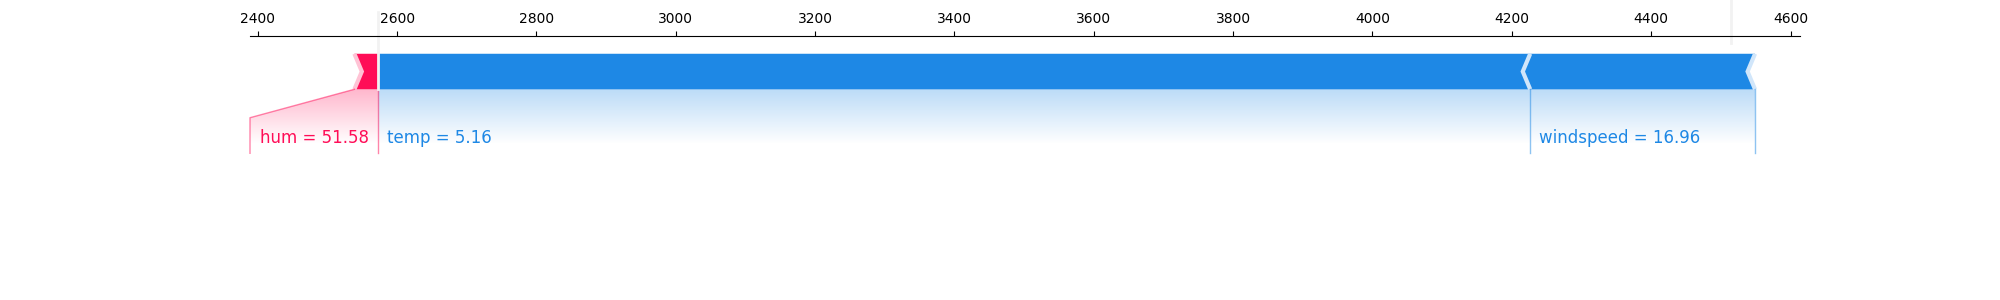
\includegraphics[width=\columnwidth]{figure_man/exSHAP.png}
%\end{figure}
%\end{frame}


\begin{frame}{Properties}

\textbf{Local Accuracy}
$$
f(\xv)=g\left(\mathbf{z}^{\prime}\right)=\phi_{0}+\sum_{j=1}^{p} \phi_{j} z_{j}^{\prime}
$$

\begin{onlyenv}<1>
\textbf{Intuition:} If the coalition includes all features ($\mathbf{z}^{\prime} = (z^{\prime}_1, \dots, z^{\prime}_p)^\top = (1, \dots, 1)^\top $), the attributions $\phi_j$ and the baseline $\phi_0$ sum up to the original model output $\fh(\xv)$\\\medskip
Local accuracy corresponds to the \textbf{axiom of efficiency} in Shapley game theory

\end{onlyenv}

\begin{onlyenv}<2->
\textbf{Missingness}
$$
z_{j}^{\prime}=0 \Longrightarrow \phi_{j}=0
$$
\end{onlyenv}

\begin{onlyenv}<2>
\textbf{Intuition:}  A "missing" feature (whose value is imputed) gets an attribution of zero
\end{onlyenv}

\begin{onlyenv}<3->
\textbf{Consistency} (Let $\mathbf{z}^{\prime (k)}_{-j} \text{ refer to } z_{j}^{\prime (k)}=0$) \\
\end{onlyenv}

\begin{onlyenv}<3>
For any two models $\fh$ and $\fh^{\prime}$, if for all inputs $\mathbf{z}^{\prime (k)} \in \{0, 1\}^p$

$$
\fh_{x}^{\prime}\left(\mathbf{z}^{\prime (k)}\right)-\fh_{x}^{\prime}\left(\mathbf{z}^{\prime (k)}_{-j}\right) \geq \fh_{x}\left(\mathbf{z}^{\prime (k)}\right)-\fh_{x}\left(\mathbf{z}^{\prime (k)} _{-j}\right) \Longrightarrow \phi_{j}\left(\fh^{\prime}, \xv\right) \geq \phi_{j}(\fh, \xv)
$$

\textbf{Intution:} If a model changes so that the marginal contribution of a feature value increases or stays the same, the Shapley value also increases or stays the same\\\medskip
From \textbf{consistency} the Shapley \textbf{axioms of additivity, dummy and symmetry} follow
\end{onlyenv}


\end{frame}

\endlecture
\end{document}
